\documentclass[10pt, a4paper]{article}
\usepackage[vmargin=1in,hmargin=1in]{geometry}
\usepackage[pdftex]{graphicx}
\usepackage{amsmath,amssymb}
\usepackage[utf8x]{inputenc}
\usepackage[english]{babel}
\usepackage[pdftex]{graphicx}
\usepackage{ctable}
\usepackage{appendix}
\usepackage{verbatim,listings}
\usepackage{epstopdf}
\usepackage{rotating}
\usepackage[lined, boxed]{algorithm2e}
\usepackage[T1]{fontenc}
\renewcommand{\familydefault}{\sfdefault} 
\newcommand{\imsize}{}
\newlength{\widthtmp}
\newcommand{\getWidth}[1]{%
  \settowidth{\widthtmp}{#1}%
  \the\widthtmp%
}
%\providecommand{\abs}[1]{\left\lvert#1\right\rvert}

\usepackage[pdftex,
pdftitle={Antidiffusion techniques to refine the numerical solution of the advection equation. Case study: Smolarkiewicz' iterative approach},
pdfauthor={G. Burger. J. Wolterink},
pdfstartview=FitH
]{hyperref}


\author{Gerhard Burger \and Jelmer Wolterink}
\title{Antidiffusion techniques to refine the numerical solution of the advection equation\\ Case study: Smolarkiewicz' iterative approach}

\newcommand{\abs}[1]{\left\lvert#1\right\rvert}

\begin{document}
\maketitle

\section{Introduction}
The advection equation describes the transport of a substance by a fluid, due to the fluid's motion in a particular direction. It plays an important role in climate modelling, e.g. in the modelling of 
\begin{itemize}
   \item Transport of trace gasses air due to wind
   \item Transport of heat by ocean water due to currents
   \item Transport of ice by ocean water due to currents
   \item Transport of warm and moist air over a colder surface by air due to wind: advection fog
\end{itemize}

A well known example of a large scale process where advection plays a role is the Thermohaline Circulation (THC). The THC advects salty water northwards in the Atlantic.

If the advection equation is solved numerically the space is discretized and this can cause diffusion. Several anti-diffusion techniques have been explored to correct for this implicit diffusion. On technique that is still in use today, be it in a generalized form, is the iterative approach developed by Smolarkiewicz in 1983 \cite{smolarki}. This approach is conceptually simple, and straightforward to implement.

In this report we will discuss the implementation of Smolarkiewicz' iterative approach in Fortran. First we will give some general remarks about numerically solving the advection equation and using anti-diffusion techniques, after that we will discuss the actual implementation and finally we will discuss some numerical results and give a short overview of the current developments in anti-diffusion techniques.

\section{Solving the advection equation}
\label{sec:solvadveq}
The continuity equation describing the advection of a non-diffusive quantity in a flow field is defined as

\begin{equation}
\frac{\partial \psi}{\partial t} + \text{ div}(V\psi) = 0
\end{equation}

where $\psi(x,y,z,t)$ is the non-diffusive scalar quantity, $V=(u,v,w)$ is the velocity vector and $x,y,z,t$ are the independent variables of space and time. In the one-dimensional case, this is 

\begin{equation}
\frac{\partial \psi}{\partial t} + \frac{\partial}{\partial x}(u\psi) = 0,
\end{equation}

To solve this partial differential equation numerically we need to take into account the following constraints on the solution:

\begin{itemize}
\item Solutions should contain no unphysical overshoot or undershoot: positive definite schemes
\item Methods should be volume preserving. No loss of matter
\item The solutions should be local: the solution at any one point should not be influenced by what is going on far away from that point
\item Methods should not introduce new extrema
\end{itemize}

\subsection{Diffusion}
Figure~\ref{fig:dif} provides a nice illustration of what diffusion in 1D is. In this example the horizontal velocity $u=0.5$ is not integral, so per time step only a portion of the quantity in the gridbox moves to the next gridbox. The red bars show the exact solution of the advection equation

\begin{equation}
 u(x,t)=F(x-ut)=F(x-0.5t).
\end{equation}

Clearly this diffusive behavior is undesirable. If your simulation runs for some time, the solution `smears' out and becomes zero everywhere. Though the solution of this method is volume preserving and no unphysical values are introduced, it is a rather bad simulation of non-diffusive advection. Furtermore, the diffusive effect extends the domain of the substance very rapidly, which could cause interactions between the substance and substances in other domains, thereby further reducing the validity of the simulation. 
\begin{figure}[htp]
\renewcommand{\imsize}{0.3\textwidth}
\begin{tabular}{ccc}
{\resizebox{\imsize}{!}{\includegraphics{../presentation/animation/anime0.pdf}}} &
{\resizebox{\imsize}{!}{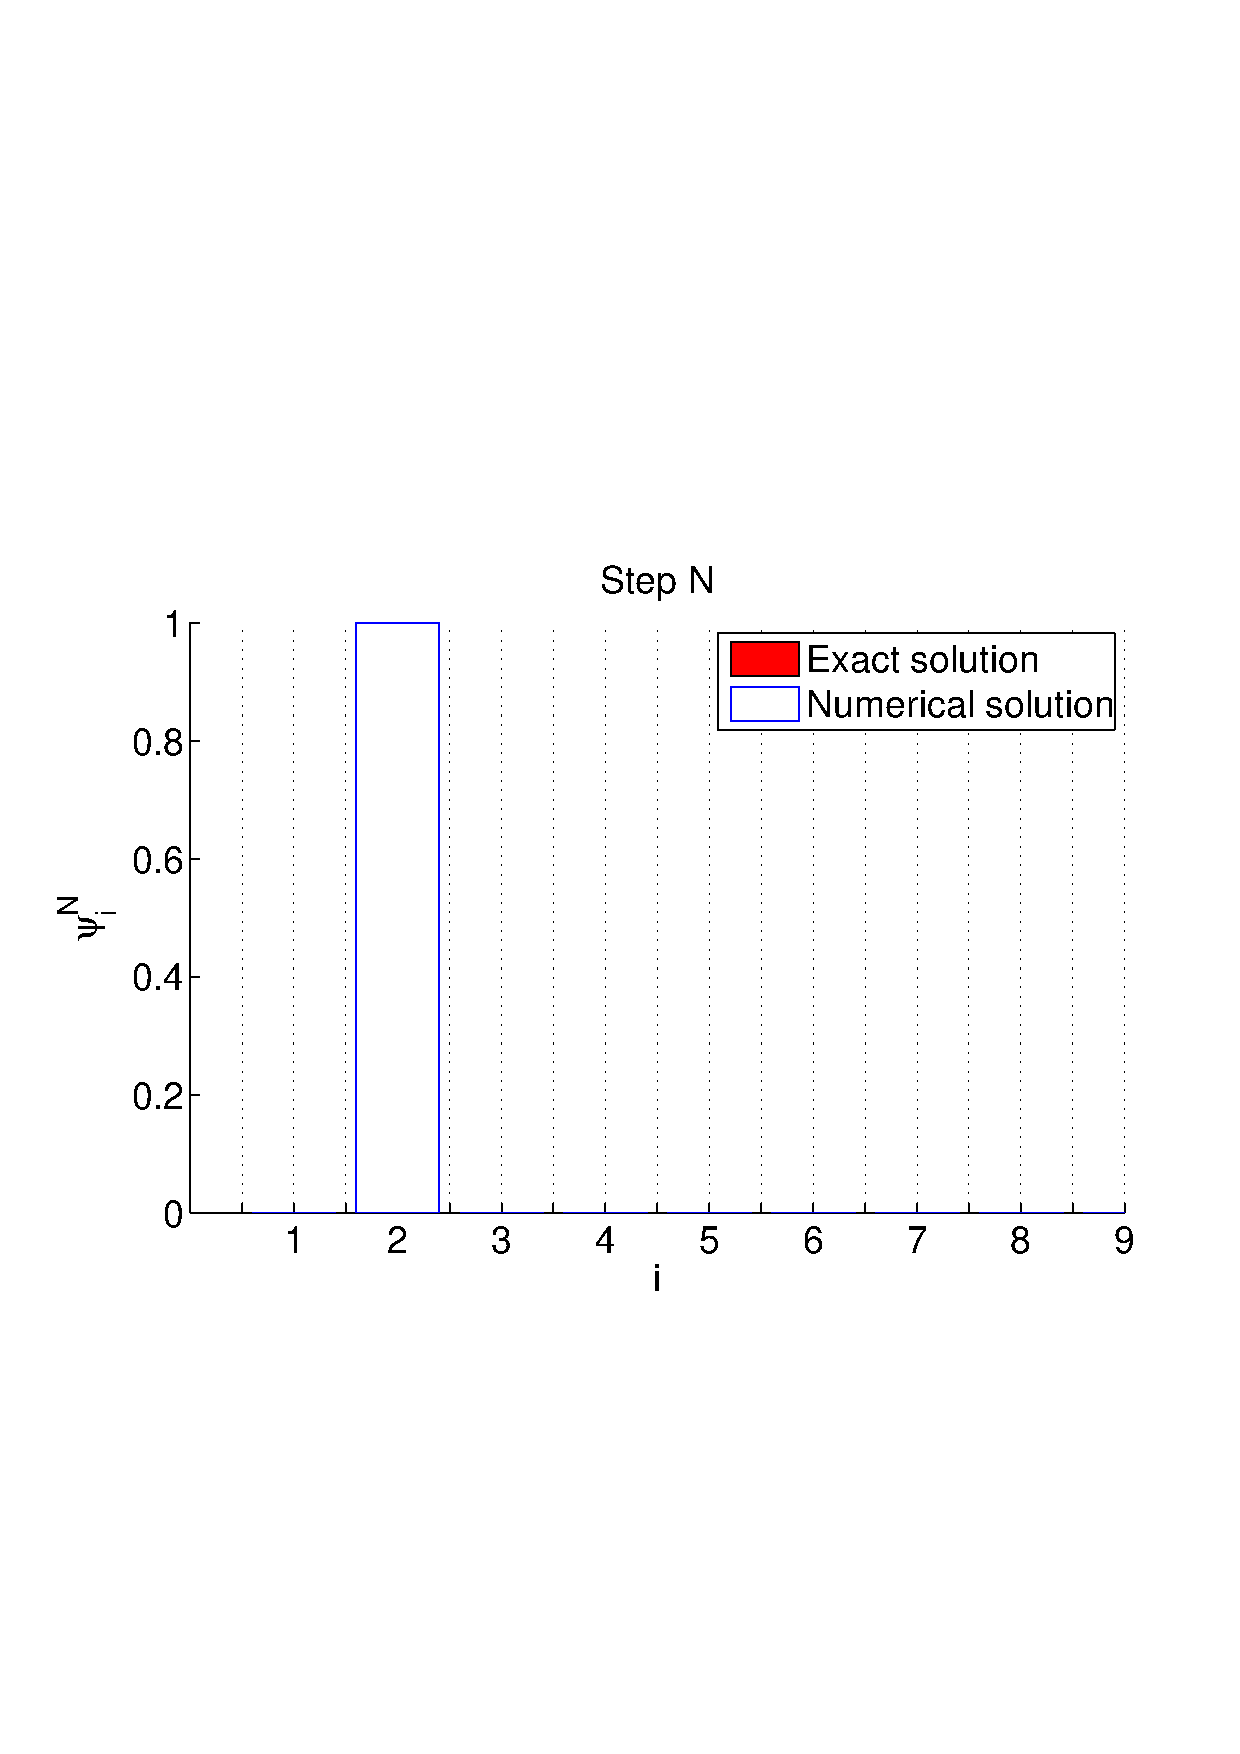
\includegraphics{../presentation/animation/anime1.pdf}}} &
{\resizebox{\imsize}{!}{\includegraphics{../presentation/animation/anime2.pdf}}} \\
{\resizebox{\imsize}{!}{\includegraphics{../presentation/animation/anime3.pdf}}} &
{\resizebox{\imsize}{!}{\includegraphics{../presentation/animation/anime4.pdf}}} &
{\resizebox{\imsize}{!}{\includegraphics{../presentation/animation/anime5.pdf}}} \\
{\resizebox{\imsize}{!}{\includegraphics{../presentation/animation/anime6.pdf}}} &
{\resizebox{\imsize}{!}{\includegraphics{../presentation/animation/anime7.pdf}}} \\
\end{tabular}
\caption{\label{fig:dif}Example of diffusion when the speed $u=0.5$.}
\label{fig:diffusion}
\end{figure}



\subsection{Anti-diffusion}
To correct for the diffusion in numerical models several techniques were proposed. There is always a trade-off between computing cost and accuracy. In \cite{smolarki}, three anti-diffusive methods are briefly introduced. The first two methods, flux-corrected transport (FCT) \cite{borisbook} and self-adjusting hybrid scheme method (SAHS) \cite{hartenzwas} share high accuracy but also require excessive computing time. Both methods calculate a weighted average of different ordered schemes to deal with diffusion. A third method by Clark and Hall \cite{clarkhall}, the hybrid-type scheme based on a Crowley advection scheme, requires less computing time but is less accurate and might introduce negative values, causing unphysical undershoot. Though these values might be small enough to be neglected, it does violate one of the contraints we set in Section \ref{sec:solvadveq}.

\section{Case study: Smolarkiewicz}
In his 1983 paper, Smolarkiewicz introduces a simple upstream scheme on a staggered grid with iterative corrections for diffusion. At every time step, a simple upstream scheme is used to calculate the advection. This results in the diffusion that we have seen in Figure \ref{fig:diffusion}. Then, the diffusive effect is reversed by a number of iterations using an antidiffusion velocity $\tilde{u}$.

In step 1 of the algorithm, Smolarkiewicz uses the upstream advection equation on a staggered grid:
\begin{equation}
 \psi_i^{N+1} = \psi_i^N - \Big( F \left( \psi_i^N,\psi_{i+1}^N,u_{i+1/2}^N\right)
-F \left( \psi_{i-1}^N,\psi_{i}^N,u_{i-1/2}^N\right) \Big),\label{eq:noanti}
\end{equation}

where

\begin{equation}
F \left( \psi_i^N,\psi_{i+1}^N,u_{i+1/2}^N\right) =
\Big( \left( u_{i+1/2}^N + \abs{u_{i+1/2}^N} \right) \psi_i^N
+ \left( u_{i+1/2}^N - \abs{u_{i+1/2}^N} \right) \psi_{i+1}^N \Big)
\frac{\Delta t}{2 \Delta x}.
\end{equation}


Here $\psi_i^N$ is the value of $\psi$ at the $i$-th grid point for time step $N$, $\Delta t$ and $\Delta x$ are the time and space incrmeents and the fluxes $F$ are defined at the same staggered points as the velocity values.

For stability we require that 

\begin{equation}
\max_{i}\left(\frac{\abs{u_{i+1/2}}\Delta t}{\Delta x}\right) \leq 1
\end{equation}

This also guarantees that the scheme is positive definite: there are no unphysical negative values in a solution at any time.

As we can see in Figure \ref{fig:diffusion}, just applying this upstream scheme will result in a highly smeared out solution after only a few steps. Therefore, in step 2 of the algorith, this upstream scheme is applied a number of times using an antidiffusive velocity, which is meant to counter the diffusion of the algorithm. We can therefore write the scheme as

\begin{align}
 \psi_i^{*} &= \psi_i^n - \Big( F \left( \psi_i^n,\psi_{i+1}^n,u_{i+1/2}^n\right)
-F \left( \psi_{i-1}^n,\psi_{i}^n,u_{i-1/2}^n\right) \Big),\label{eq:anti1}\\
 \psi_i^{n+1} &= \psi_i^* - \Big( F \left( \psi_i^*,\psi_{i+1}^*,\tilde{u}_{i+1/2}^n\right)
-F \left( \psi_{*}^n,\psi_{*}^n,\tilde{u}_{i-1/2}^n\right) \Big),\label{eq:anti2}\,
\end{align} 

where

\begin{equation}
\tilde{u}_{i+1/2} = \frac{\left(\abs{u_{i+1/2}}\Delta x - \Delta t u_{i+1/2}^2 \right) \left( \psi_{i+1}^*-\psi_i^*\right)}{ \left( \psi_i^*+\psi_{i+1}^*+\epsilon \right) \Delta x}
\end{equation}

We see that \ref{eq:anti1} is the same as \ref{eq:noanti}, only now the result is not directly stored in $\psi^{N+1}$, but in an intermediate vector $\psi^*$. Then we can apply \ref{eq:anti2} any number of times to increase the accuracy of the simulation. In practice, the gain in accuracy decreases with the number of iterations. The exact number of iterations to use depends on the computational resources at hand, Smolarkiewicz suggests using 2 iterations.

\subsection{Implementation}
We implement the antidiffusion scheme in Fortran. For this, we use the method of lines. First, we write out the equations. We see that \ref{eq:anti1} and \ref{eq:anti2} use the same flux operators, only the input velocity vector and system state vector are different. Therefore, we only need to write out \ref{eq:anti1}.

\begin{multline}
\psi_i^* = \psi_i^N - \frac{\Delta t}{2 \Delta x} \bigg( \Big( \left( u_{i+1/2}^N + \abs{u_{i+1/2}^N} \right) \psi_i^N
+ \left( u_{i+1/2}^N - \abs{u_{i+1/2}^N} \right) \psi_{i+1}^N \Big)
\\
- \Big( \left( u_{i-1/2}^N + \abs{u_{i-1/2}^N} \right) \psi_{i-1}^N
+ \left( u_{i-1/2}^N - \abs{u_{i-1/2}^N} \right) \psi_{i}^N \Big) \bigg).
\end{multline}
Collecting terms gives the method of lines representation
\begin{equation}
\begin{split}
\psi_i^* &=
\frac{\Delta t}{2 \Delta x} \left( u_{i-1/2}^N + \abs{u_{i-1/2}^N} \right) \psi_{i-1}^N\\
&+ \left(1 - \frac{\Delta t}{2 \Delta x} \left( u_{i+1/2}^N + \abs{u_{i+1/2}^N} - u_{i-1/2}^N + \abs{u_{i-1/2}^N} \right) \right) \psi_i^N\\
&-\frac{\Delta t}{2 \Delta x} \left( u_{i+1/2}^N - \abs{u_{i+1/2}^N} \right) \psi_{i+1}^N\\
\end{split}
\end{equation}

With substitution of terms

\begin{equation*}
\psi_i^* = \alpha_i \psi_{i-1}^N + \beta_i \psi_i^N +\gamma_i \psi_{i+1}^N, \quad \text{for } i=1,\ldots,M-1,
\end{equation*}
 where we have that
\begin{align*}
\alpha_i &= \frac{\Delta t}{2 \Delta x} \left( u_{i-1/2}^N + \abs{u_{i-1/2}^N} \right),\\
 \beta_i &= \left(1 - \frac{\Delta t}{2 \Delta x} \left( u_{i+1/2}^N + \abs{u_{i+1/2}^N} - u_{i-1/2}^N + \abs{u_{i-1/2}^N} \right) \right),\\
\gamma_i &= -\frac{\Delta t}{2 \Delta x} \left( u_{i+1/2}^N - \abs{u_{i+1/2}^N} \right).
\end{align*}

We can write this in matrix form using Dirichlet boundary conditions as

\begin{equation*}
\begin{bmatrix}\psi_{1}^*\\\psi_{2}^*\\ \vdots \\\psi_{M-2}^*\\\psi_{M-1}^*\end{bmatrix} =
\begin{bmatrix}\beta_1&\gamma_1&&&0\\ \alpha_2&\beta_2&\gamma_2\\ &\ddots&\ddots&\ddots\\&&\alpha_{M-2}&\beta_{M-2}&\gamma_{M-2}\\0&&&\alpha_{M-1}&\beta_{M-1}\\ \end{bmatrix}
\begin{bmatrix}\psi_{1}^N\\\psi_{2}^N\\ \vdots \\\psi_{M-2}^N\\\psi_{M-1}^N\end{bmatrix}
\end{equation*}

or with periodic boundary conditions, so that we only need to store a limited domain for long simulations, as

\begin{equation*}
\begin{bmatrix}\psi_{1}^*\\\psi_{2}^*\\ \vdots \\\psi_{M-2}^*\\\psi_{M-1}^*\end{bmatrix} =\begin{bmatrix}\beta_1&\gamma_1&&&\mathbf{\alpha_1}\\ \alpha_2&\beta_2&\gamma_2\\ &\ddots&\ddots&\ddots\\&&\alpha_{M-2}&\beta_{M-2}&\gamma_{M-2}\\ \mathbf{\gamma_{M-1}}&&&\alpha_{M-1}&\beta_{M-1}\\ \end{bmatrix}
\begin{bmatrix}\psi_{1}^N\\\psi_{2}^N\\ \vdots \\\psi_{M-2}^N\\\psi_{M-1}^N\end{bmatrix}
\end{equation*}

The values of $\psi^*$ can be obtained very efficiently from those of $\psi^N$ using a sparse matrix vector multiplication. It follows that we can apply this matrix-vector multiplication also to \ref{eq:anti2}, where we substitute $u \rightarrow \tilde{u}$, $\psi^N \rightarrow \psi^*$, $\psi^* \rightarrow \psi^{N+1}$ in case we only run one iteration of \ref{eq:anti2}. If we run more than one iteration, we should update the intermediate vector $\psi^*$ and the antidiffusion velocity $\tilde{u}$ at each iteration.

Note that the tri-diagonal matrix is only useful for the one dimensional case. If we apply Smolarkiewicz' antidiffusion scheme in two dimensions, we need to take into account two extra neighboring grid points for every grid point $\psi_{ij}$. Thus, we get the collection of terms 

\begin{align*}
\psi_{ij}^* &=
\frac{\Delta t}{2 \Delta y} \left( v_{i,j-1/2}^N + \abs{v_{i,j-1/2}^N} \right) \psi_{i,j-1}^N\\
&+\frac{\Delta t}{2 \Delta x} \left( u_{i-1/2,j}^N + \abs{u_{i-1/2,j}^N} \right) \psi_{i-1,j}^N\\
&+ \Big(1 - u_{i+1/2,j}^N - \abs{u_{i+1/2,j}^N} + u_{i-1/2,j}^N - \abs{u_{i-1/2,j}^N} - v_{i,j+1/2}^N - \abs{v_{i,j+1/2}^N} \\
&+ v_{i,j-1/2}^N - \abs{v_{i,j-1/2}^N} \Big) \psi_i^N\\
&-\frac{\Delta t}{2 \Delta x} \left( u_{i+1/2,j}^N - \abs{u_{i+1/2,j}^N} \right) \psi_{i+1,j}^N\\
&-\frac{\Delta t}{2 \Delta y} \left( v_{i,j+1/2}^N - \abs{v_{i,j+1/2}^N} \right) \psi_{i,j+1}^N,\\
\end{align*}

substitution gives

\begin{align*}
\alpha_i &= \frac{\Delta t}{2 \Delta y} \left( v_{i,j-1/2}^N + \abs{v_{i,j-1/2}^N} \right),\\
\beta_i &= \frac{\Delta t}{2 \Delta x} \left( u_{i-1/2,j}^N + \abs{u_{i-1/2,j}^N} \right),\\
\gamma_i &= \Big(1 - u_{i+1/2,j}^N - \abs{u_{i+1/2,j}^N} + u_{i-1/2,j}^N - \abs{u_{i-1/2,j}^N} - v_{i,j+1/2}^N - \abs{v_{i,j+1/2}^N} \\
&+ v_{i,j-1/2}^N - \abs{v_{i,j-1/2}^N} \Big),\\
\delta_i &= -\frac{\Delta t}{2 \Delta x} \left( u_{i+1/2,j}^N - \abs{u_{i+1/2,j}^N} \right),\\
\epsilon_i &= -\frac{\Delta t}{2 \Delta y} \left( v_{i,j+1/2}^N - \abs{v_{i,j+1/2}^N} \right).
\end{align*}

\begin{equation*}
\psi_{ij}^* = \alpha_{ij} \psi_{i,j-1}^N + \beta_{ij} \psi_{i-1,j}^N +\gamma_{ij} \psi_{i,j}^N +\delta_{ij} \psi_{i+1,j}^N + \epsilon_{ij} \psi_{i,j+1}^N, \quad \text{for } i,j=1,\ldots,M-1,
\end{equation*}

which gives a pentadiagonal sparse matrix. Again, we can use sparse matrix vector multiplication. In the three-dimensional case, we would get a septadiagonal matrix.

In general, we find a numerical solution using the following algorithm

\IncMargin{1em}
\begin{algorithm}[H]
\SetKwData{Iter}{iter}\SetKwData{Mone}{mat1}\SetKwData{Mtwo}{mat2}
\SetKwData{Steps}{tsteps}
\SetKwFunction{MMat}{ComputeMatrix}\SetKwFunction{MMult}{MatrixMultiplication}
\SetKwFunction{CADV}{ComputeAntidiffusionVelocity}
\SetKwInOut{Input}{input}\SetKwInOut{Output}{output}
\Input{Initial state $\psi^0$, velocities $u$, \Iter, \Steps, $\Delta x$, $\Delta t$} 
\Output{Final state $\psi^N$}
\BlankLine
$\psi \leftarrow \psi^0$\;
\Mone $\leftarrow$ \MMat{$u,\Delta x, \Delta t$}\;
\For{$i \leftarrow 1$ \KwTo \Steps}{
$\psi \leftarrow$ \MMult{\Mone,$\psi$}\;
\For{$j \leftarrow 1$ \KwTo \Iter}{
$\widetilde{u} \leftarrow$ \CADV{$\psi,u$}\;
\Mtwo $\leftarrow$ \MMat{$\widetilde{u},\Delta x, \Delta t$}\;
$\psi \leftarrow$ \MMult{\Mtwo,$\psi$}\;
}
}
$\psi^N \leftarrow \psi$\;
\end{algorithm}
\DecMargin{1em}





\subsection{Numerical results}
We have applied the antidiffusive scheme to the one dimensional case and the two dimensional case. We will first discuss some results for the one dimensional case.


\subsubsection{Results in one dimension}
We have developed a graphical user interface (GUI) in Matlab (Figure \ref{fig:1dgui}) so that we can test different configurations on the fly. In the GUI, we can check for instabilities and set the initial condition and the velocity vector very easily. Using this GUI we find that the scheme is indeed both volume preserving and positive definite. 

We can visualize the effect of using antidiffusion iterations by again taking the problem in Figure \ref{fig:dif}, but now applying two antidiffusion iterations at each timestep. In the blue bars, we have the original diffused 

\begin{figure}[htp]
\renewcommand{\imsize}{0.3\textwidth}
\begin{tabular}{ccc}
{\resizebox{\imsize}{!}{\includegraphics{../presentation/animation/aanime0-eps-converted-to.pdf}}} &
{\resizebox{\imsize}{!}{\includegraphics{../presentation/animation/aanime1-eps-converted-to.pdf}}} &
{\resizebox{\imsize}{!}{\includegraphics{../presentation/animation/aanime2-eps-converted-to.pdf}}} \\
{\resizebox{\imsize}{!}{\includegraphics{../presentation/animation/aanime3-eps-converted-to.pdf}}} &
{\resizebox{\imsize}{!}{\includegraphics{../presentation/animation/aanime4-eps-converted-to.pdf}}} &
{\resizebox{\imsize}{!}{\includegraphics{../presentation/animation/aanime5-eps-converted-to.pdf}}} \\
{\resizebox{\imsize}{!}{\includegraphics{../presentation/animation/aanime6-eps-converted-to.pdf}}} &
{\resizebox{\imsize}{!}{\includegraphics{../presentation/animation/aanime7-eps-converted-to.pdf}}} \\
\end{tabular}
\caption{\label{fig:antidif}Example of antidiffusion when the speed $u=0.5$.}
\label{fig:diffusion}
\end{figure}


Furthermore, we find that when we use antidiffusive iterations, the diffusion is much smaller than in the case where we just apply the basic upstream scheme. We see this very clearly in Figure \ref{fig:maxs}, where we have plotted the maximum value of the simulation as a function of the time step $N$. When we do not use antidiffusion, the maximum value rapidly drops to 0, when we use 3 antidiffusion iterations, the maximum value drops to 0.5, but then remains constant around that value. In this example, the move from 2 to 3 antidiffusion iterations adds relatively little to the validity of the simulation, compared to the extra computational cost.

In Figure \ref{fig:local} we see that without antidiffusion iterations, 

\begin{figure}
\centering
 \includegraphics[width=0.8\textwidth]{1dscreenshot.png}
 \caption{Matlab GUI for one dimensional case. We can set the velocity vector $u$, the initial condition $\psi^0$ and a range of other parameters.}
 \label{fig:1dgui}
\end{figure}

\begin{figure}
\centering
 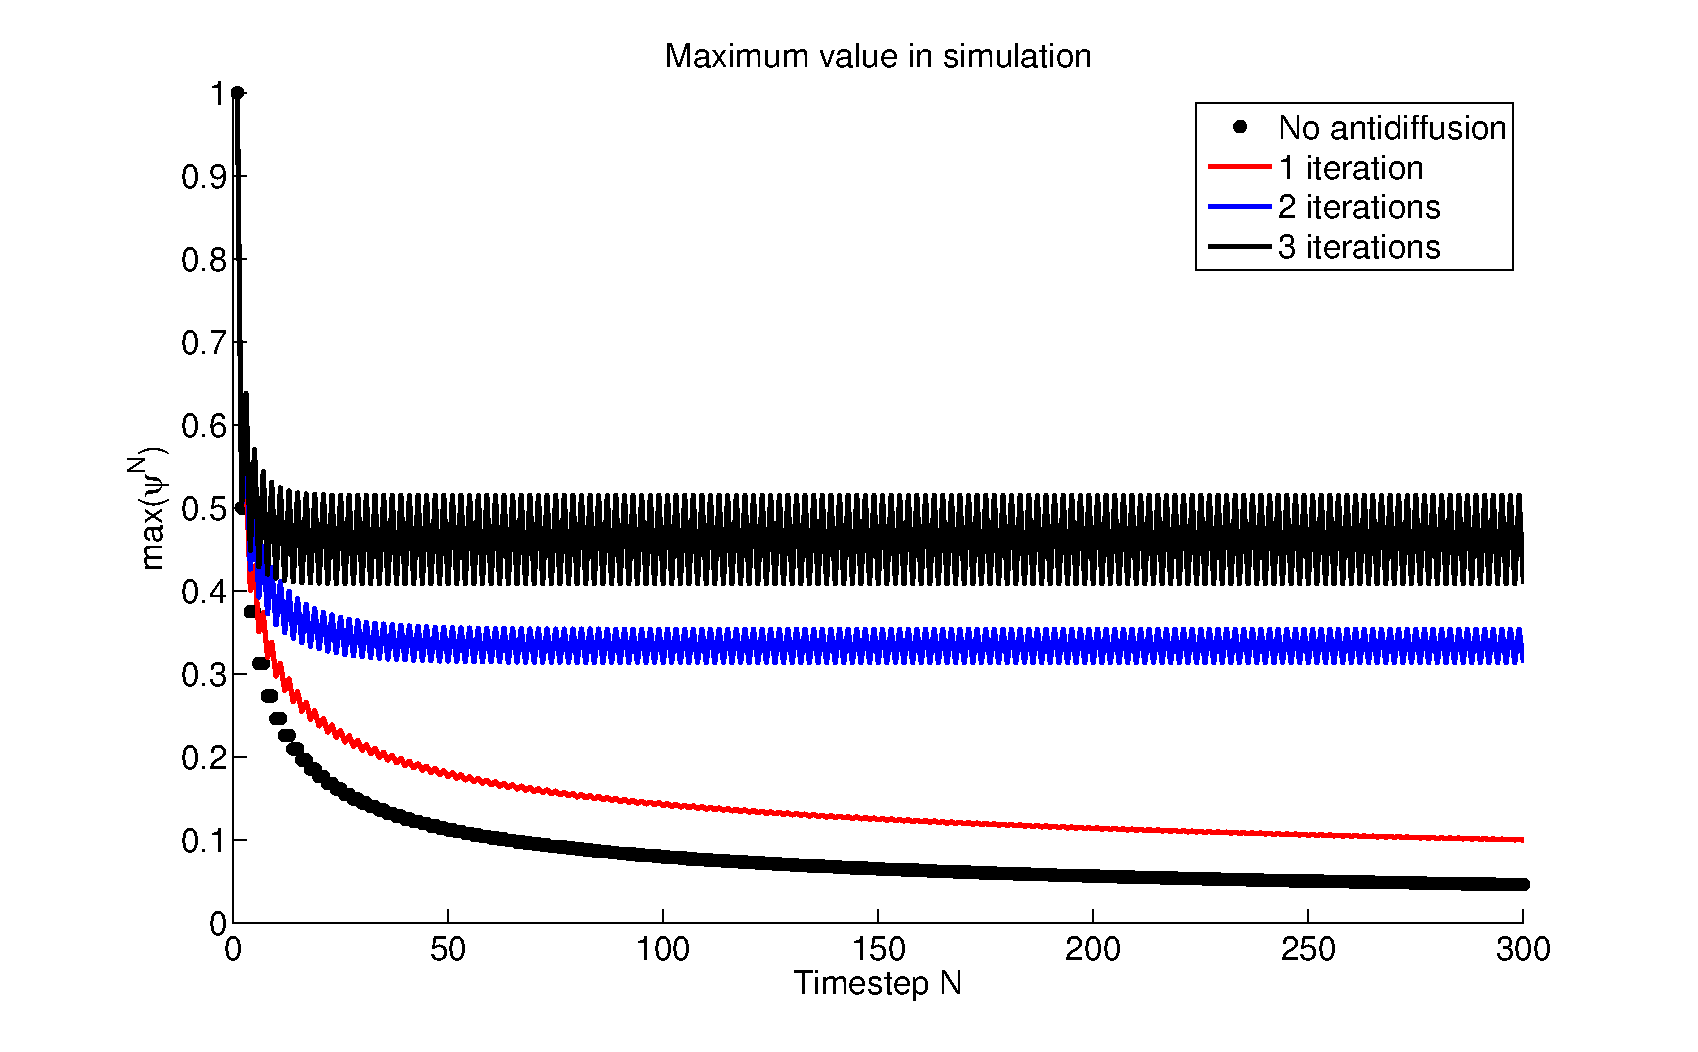
\includegraphics[width=0.8\textwidth]{maxs}
 \caption{Maximum value in the simulation when running with 0, 1, 2 or 3 antidiffusive iterations.}
 \label{fig:maxs}
\end{figure}

\begin{figure}
\centering
 \includegraphics[width=0.8\textwidth]{2dscreenshot.jpg}
 \caption{Matlab GUI for two dimensional case. We can set the velocity vectors $u$ and $v$, the initial condition $\psi^0$ and a range of other parameters. We can view the results of the simulation directly.}
 \label{fig:2dgui}
\end{figure}

\subsubsection{Results in two dimensions}

In both cases it is interesting to vi
\section{Current state of research}
Something about no diffusion schemes
\subsection{Possibilities}
\subsection{MPDATA}
\section{Conclusion}




Collecting terms gives the method of lines representation

\begin{equation}
\begin{split}
\psi_{ij}^{N+1} &=
\frac{\Delta t}{2 \Delta y} \left( v_{i,j-1/2}^N + \abs{v_{i,j-1/2}^N} \right) \psi_{i,j-1}^N\\
&+\frac{\Delta t}{2 \Delta x} \left( u_{i-1/2,j}^N + \abs{u_{i-1/2,j}^N} \right) \psi_{i-1,j}^N\\
&+ \Big(1 - u_{i+1/2,j}^N - \abs{u_{i+1/2,j}^N} + u_{i-1/2,j}^N - \abs{u_{i-1/2,j}^N} - v_{i,j+1/2}^N - \abs{v_{i,j+1/2}^N} \\
&+ v_{i,j-1/2}^N - \abs{v_{i,j-1/2}^N} \Big) \psi_i^N\\
&-\frac{\Delta t}{2 \Delta x} \left( u_{i+1/2,j}^N - \abs{u_{i+1/2,j}^N} \right) \psi_{i+1,j}^N\\
&-\frac{\Delta t}{2 \Delta y} \left( v_{i,j+1/2}^N - \abs{v_{i,j+1/2}^N} \right) \psi_{i,j+1}^N\\
\end{split}
\end{equation}

\bibliographystyle{plain}
\bibliography{report}

\end{document}
